\documentclass[letterpaper]{article}
\usepackage{flairs}%aaai
\usepackage{times}
\usepackage{helvet}
\usepackage{courier}
\usepackage{graphicx}
\usepackage{setspace}
\usepackage{url}
\frenchspacing
\setlength{\pdfpagewidth}{8.5in}
\setlength{\pdfpageheight}{11in}
\pdfinfo{
/Title (The Interactive Interpretation Viewer)
/Author (Jack McKeown, Geoff Sutcliffe)} 

\setcounter{secnumdepth}{2}  

%----Making things more compact
\newcommand{\smalltt}[1]{\small \texttt{#1}}
\newenvironment{packed_itemize}{
\vspace*{-0.2em}
\begin{itemize}
\setlength{\partopsep}{0pt}
\setlength{\itemsep}{1pt}
\setlength{\parskip}{0pt}
\setlength{\parsep}{0pt}
}{\end{itemize}}
\newenvironment{packed_enumerate}{
\vspace*{-0.2em}
\begin{enumerate}
\setlength{\partopsep}{0pt}
\setlength{\itemsep}{1pt}
\setlength{\parskip}{0pt}
\setlength{\parsep}{0pt}
}{\end{enumerate}}
\renewcommand{\textfraction}{0.07}
\renewcommand{\topfraction}{0.9}
\renewcommand{\bottomfraction}{0.9}
\renewcommand{\floatpagefraction}{0.66}
\setlength{\floatsep}{2.0pt plus 2.0pt minus 2.0pt}
\setlength{\textfloatsep}{5.0pt plus 2.0pt minus 0.0pt}

\begin{document}

\title{The Interactive Interpretation Viewer}
\author{Anon One\\
Some where\\
Some place\\
Some country\\
\And
Anon Two\\
Some where\\
Some place\\
Some country}

\maketitle
\begin{abstract}
\begin{quote}
This poster describes IIV.
\end{quote}
\end{abstract}
%--------------------------------------------------------------------------------------------------
\section{Introduction}
\label{Introduction}

Automated Reasoning (AR), and Automated Theorem Proving (ATP) in particular, has focused largely 
on the task of proving theorems from axioms -- the derivation of conclusions that follow inevitably 
from known facts \cite{RV01-HAR}.
The axioms and conjecture to be proved (and hence become a theorem) are written in an 
appropriately expressive logic, and the proofs are often similarly written in logic \cite{SS+06}.
In this work typed first-order logic is used.
In the last two decades the converse task of disproving conjectures
has become increasingly important.
This process depends on finding an {\em interpretation}, i.e., a structure that maps terms 
to domain elements and formulae to truth values.
An interpretation that maps a formula to {\em true} is a {\em model} of the formula.
A conjecture is disproved by finding an interpretation that is a model of the axioms, but 
maps the conjecture to {\em false}.
A salient application area that harnesses this form of ATP is verification \cite{DKW08},
where a countermodel is used to pinpoint the reason why a proof obligation fails, and
correspondingly points to the location of the fault in the system being verified.
This work describes an interactive interpretation viewer for interpretations written in the
(new) TPTP format for interpretations \cite{FLAIRS}.

\paragraph{Related Work:}
Related work is sparse.
The Mace4 model finder \cite{McC03-MACE4-TR} outputs textual 
information about the models it finds, including the interpretation of constants as integers,
and tables for the function and predicate symbols' interpretations. 
The tables are naturally limited to symbols of arity up to two (which is just fine for algebras, 
where Mace4 is often applied).
The only graphical visualization tool that has been found is that described in \cite{Sch13-MS},
which provided (past tense -- it is no longer available) a visualization of finite first-order 
interpretations as produced by Paradox.
The visualization had some nice features, e.g., showing functions as constructor functions, and 
reducing the visual clutter when displaying relations with properties such as symmetry, 
transitivity, etc.
In other ways that work was quite different from the visualization described in this work.

%--------------------------------------------------------------------------------------------------
\section{The TPTP World and Languages}
\label{TPTP}

The TPTP World \cite{Sut17} is a well established infrastructure that supports research, 
development, and deployment of Automated Theorem Proving (ATP) systems.
The TPTP language \cite{Sut22-IGPL} is one of the keys to the success of the TPTP World.
The language is used for writing both problems and solutions.
The top level building blocks of the TPTP language are {\em annotated formulae}.
An annotated formula has the form:\\
\hspace*{0.5cm}{\em language}{\tt (}{\em name}{\tt ,}
{\em role}{\tt ,}
{\em formula}{\tt ,}
{\em source}{\tt ,}
{\em useful\_info}{\tt )}\\
The {\em language}s supported are {\smalltt{cnf}} (clause normal form), {\smalltt{fof}}
(first-order form), {\smalltt{tff}} (typed first-order form), and {\smalltt{thf}}
(typed higher-order form).
The {\em role}, e.g., {\smalltt{axiom}}, {\smalltt{lemma}}, {\smalltt{conjecture}},
defines the use of the formula in an ATP system.
In a {\em formula}, terms and atoms follow Prolog conventions
-- functions and predicates start with a lowercase letter or are {\tt '}single quoted{\tt '}, and 
variables start with an uppercase letter.
The language also supports interpreted symbols, which either start with a {\tt \$}, e.g., 
the truth constants {\smalltt{\$true}} and {\smalltt{\$false}}, or are composed of 
non-alphanumeric characters, e.g., integer/rational/real numbers such as 27, 43/92, -99.66.
The basic logical connectives are
{\tt !}, {\tt ?}, {\tt \verb|~|}, {\tt |}, {\tt \&}, {\tt =>}, {\tt <=}, {\tt <=>}, and 
{\tt <{\raisebox{0.4ex}{\texttildelow}}>},
for
$\forall$, $\exists$, $\neg$, $\vee$, $\wedge$, $\Rightarrow$, $\Leftarrow$, $\Leftrightarrow$, 
and $\oplus$ respectively.
Equality and inequality are expressed as the infix operators {\tt =} and {\tt !=}.
The {\em source} and {\em useful\_info} are optional.
Figure~\ref{TF0FiniteProblem} is an example of a problem in monomorphic typed first-order
form (TF0).  
The associated (counter)model is discussed in Section~\ref{Interpretations}.

\begin{figure}[htbp]
\scriptsize
\setstretch{0.8}
\begin{verbatim}
%--------------------------------------------------------
tff(man_type,type,           man: $tType ).
tff(grade_type,type,         grade: $tType ).
tff(john_decl,type,          john: man ).
tff(a_decl,type,             a: grade ).
tff(f_decl,type,             f: grade ).
tff(grade_of_decl,type,      grade_of: man > grade ).
tff(created_equal_decl,type, 
    created_equal: ( man * man ) > $o ).

tff(all_created_equal,axiom,
    ! [H1: man,H2: man] : created_equal(H1,H2) ).

tff(john_failed,axiom,
    grade_of(john) = f ).

tff(someone_got_an_a,axiom,
    ? [H: man] : grade_of(H) = a ).

tff(distinct_grades,axiom,
    a != f ).

tff(equality_lost,conjecture,
    ! [H1: man,H2: man] :
      ( created_equal(H1,H2) <=> ( H1 = H2 ) ) ).
%--------------------------------------------------------
\end{verbatim}
\caption{A TF0 problem (with a finite countermodel)\\
{\scriptsize \url{https://raw.githubusercontent.com/GeoffsPapers/ModelVerification/main/TFF_Finite.p}}}
\label{TF0FiniteProblem}
\end{figure}

%--------------------------------------------------------------------------------------------------
\section{Interpretations}
\label{Interpretations}

A Tarskian-style interpretation \cite{TV56} of formulae in typed first-order logic consists of a 
non-empty domain of unequal elements for each type used in the formulae (just one domain for 
untyped logic), and interpretations of the function and predicate symbols with respect to the 
domains \cite{Hun96}.
The domains of an interpretation may be finite or infinite.
Interpretations with only finite domains are called {\em finite interpretations}, and
interpretations with one of more infinite domains are called {\em infinite interpretations}.
Finite domains are commonly explicitly enumerated, but can also take other forms, e.g., the 
finite Herbrand Universe of a Herbrand interpretation \cite{Her30}.
Infinite domains can take several forms, including being implicitly specified (e.g., some set
of algebraic numbers, such as the integers), explicitly generated (e.g., terms representing 
Peano numbers), and the infinite Herbrand Universe of a Herbrand interpretation.

The underlying principle is to represent interpretations as formulae.
The representation format uses an {\em interpretation formula}, preceded by the necessary type 
declarations.
%\begin{packed_itemize}
%\item the type declarations for the formulae being interpreted;
%\item the types of the domains (unless already defined in the language, e.g., the type
%      {\smalltt{\$int}});
%\item the types of type-promotion functions from the types of the domains to the types 
%      of the formulae, used to make the interpretation formula well-typed;
%\item the types of the domain elements.
%\end{packed_itemize}
% \vspace*{-0.4em}
The interpretation formula is a conjunction specifying: 
\begin{packed_itemize}
\item for each type in the formulae:
      \begin{packed_itemize}
      \item the domain type, by a formula that makes the type-promotion function a surjection;
      \item the domain elements as a universally quantified disjunction of equalities whose 
            right-hand sides are the domain elements;
      \item specification of the distinctness of the domain elements;
      \item a formula making the type-promotion function an injection,
            which with the surjectivity makes it a bijection.
      \end{packed_itemize}
\item interpretation of the function symbols, as equalities whose left-hand sides are 
      formed from symbols applied to type-promoted domain elements, and whose right-hand sides 
      are type-promoted domain elements;
\item interpretation of the predicate symbols, as literals formed from symbols applied
      to type-promoted domain elements; positive literals are {\em true} and negative literals 
      are {\em false}.
\end{packed_itemize}
This representation is also directly usable for untyped first-order logic, where all terms in 
the given and interpretation formulae are of the same type – ``individuals''. 
This obviates the need for type considerations, in particular type-promotion functions are not 
needed.

Figure~\ref{TF0FiniteInterpretation} is a TF0 interpretation with finite domains -- it is a 
countermodel for the problem in Figure~\ref{TF0FiniteProblem}.
The comments show which parts of the formula specify what aspects of the interpretation, per
the list above.

\begin{figure}[t!]
\scriptsize
\setstretch{0.8}
\begin{verbatim}
%--------------------------------------------------------
tff(man_type,type,           man: $tType ).
tff(grade_type,type,         grade: $tType ).
tff(john_decl,type,          john: man ).
tff(a_decl,type,             a: grade ).
tff(f_decl,type,             f: grade ).
tff(grade_of_decl,type,      grade_of: man > grade ).
tff(created_equal_decl,type, 
    created_equal: ( man * man ) > $o ).

%----Types of the domains
tff(d_man_type,type,         d_man: $tType).
tff(d_grade_type,type,       d_grade: $tType).
%----Types of the promotion functions
tff(d2man_decl,type,         d2man: d_man > man ).
tff(d2grade_decl,type,       d2grade: d_grade > grade ).
%----Types of the domain elements
tff(d_john_decl,type,        d_john: d_man ).
tff(d_gotA_decl,type,        d_gotA: d_man ).
tff(d_a_decl,type,           d_a: d_grade ).
tff(d_f_decl,type,           d_f: d_grade ).

tff(equality_lost,interpretation,
%----The domain for man is d_man
    ( ( ! [M: man] : ? [DM: d_man] : M = d2man(DM)
%----The d_man elements are d_john and d_gotA
      & ! [DM: d_man] : ( DM = d_john | DM = d_gotA )
      & $distinct(d_john,d_gotA)
%----The type-promoter is a bijection
      & ! [DM1: d_man,DM2: d_man] :
          ( d2man(DM1) = d2man(DM2) => DM1 = DM2 )
%----The domain for grade is d_grade
      & ! [G: grade] : ? [DG: d_grade] : G = d2grade(DG)
%----The d_grade elements are d_a and d_f
      & ! [DG: d_grade]: ( DG = d_a | DG = d_f )
      & $distinct(d_a,d_f)
%----The type-promoter is a bijection
      & ! [DG1: d_grade,DG2: d_grade] :
          ( d2grade(DG1) = d2grade(DG2) => DG1 = DG2 ) )
%----Interpret terms via the type-promoted domain
    & ( a = d2grade(d_a)
      & f = d2grade(d_f)
      & john = d2man(d_john)
      & grade_of(d2man(d_john)) = d2grade(d_f)
      & grade_of(d2man(d_gotA)) = d2grade(d_a) )
%----Interpret atoms as true of false
    & ( created_equal(d2man(d_john),d2man(d_john))
      & created_equal(d2man(d_john),d2man(d_gotA))
      & created_equal(d2man(d_gotA),d2man(d_john))
      & created_equal(d2man(d_gotA),d2man(d_gotA)) ) 
    ) ).
%--------------------------------------------------------
\end{verbatim}
\caption{A TF0 interpretation with a finite domain \\
{\scriptsize \url{https://raw.githubusercontent.com/GeoffsPapers/ModelVerification/main/TFF_Finite.s}}}
\label{TF0FiniteInterpretation}
\end{figure}

%--------------------------------------------------------------------------------------------------
\section{Interpretation Visualization}
\label{Visualization}

Proof visualization is well-established, with several tools available, e.g., 
Evonne \cite{AB+22},
%  is an interactive proof visualization software for description logics,
% \footnote{\smalltt{https://lat.inf.tu-dresden.de/research/papers/2022/ALBABODAKOME-IJCAR22.pdf}}
ProofTree \cite{Tew17},
% is a proof visualization tool focused on interactive theorem proving within Coq,
% \footnote{\smalltt{https://askra.de/software/prooftree/}} 
% ProofTree currently only supports proofs from Coq.
Treehehe \cite{Bat18},
%  was designed generically to visualize any proof tree,
% \footnote{\smalltt{https://chelsea.lol/Resources/COMP5209\_BattellC\_report.pdf}} 
% but currently it only supports a handful of pre-existing proofs and does not allow users 
%to visualize their own proofs.
and
the Interactive Derivation Viewer \cite{TPS07} (IDV) -- a tool for visualization of 
TPTP format proofs.
Interpretation visualization, however, has (to the knowledge of the authors) had minimal 
attention, as noted in Section~\ref{Introduction}. 
Visualization of interpretations is useful in areas such as teaching logic, debugging ATP 
systems, and understanding of a model.

A visualization for TF0 interpretations has been designed in this work, and an initial
implementation is available as the IIV tool in the SystemOnTSTP web interface.
IIV is built on top of IDV, and has benefited from the mature state of IDV.
% IDV was originally a Java applet, but has since been ported to HTML/JavaScript using GraphViz
% \cite{EG+02} for the layout and rendering.
% IIV has benefited from the mature state of IDV.
The implementation is ``initial'' because it is fully automated for only finite TF0
interpretations; for infinite interpretations different components of the interpretation formula 
have to be manually extracted into separate annotated formulae, to mimic a derivation that IDV 
can render.

Figure~\ref{TF0FiniteIIV} is the visualization of the finite countermodel in 
Figure~\ref{TF0FiniteInterpretation}, modified so that {\smalltt{john}} is not created equal 
to the person who got an {\smalltt{A}}.
The top row of inverted triangles are the types in the given formulae,
while the bottom row of inverted triangles are the types of the domains in the interpretation
formula.
The inverted houses are the function and predicate symbols, and the successive rows of ovals are 
the successive domain element arguments used to specify the symbols' interpretation.
Finally, the row of houses and boxes are the interpretations of the symbols applied to those
arguments; houses for functions and boxes for predicates.
For example, in the given formulae the type of {\smalltt{grade\_of}} is {\smalltt{grade}},
and {\smalltt{grade\_of(d\_john)}} is interpreted as {\smalltt{d\_f}}, which is of type
{\smalltt{d\_grade}} in the interpretation formula.

IIV provides some interactive features: Figure~\ref{TF0FiniteIIV} shows the situation with 
the cursor hovering over the lower {\smalltt{d\_john}} node on the path from 
{\smalltt{created\_equal}} to {\smalltt{\$true}}, showing that
{\smalltt{created\_equal(d\_john,d\_john)}} is interpreted as {\smalltt{\$true}}.
The nodes above are increasingly darker red (grey if printed) up to the type node {\smalltt{\$o}} 
that is the result type of {\smalltt{created\_equal}}, and increasingly darker blue down to 
the type node {\smalltt{\$o}} that is the type of {\smalltt{\$true}}.
This highlighting provides easy focus on the interpretations of chosen symbols.
% inverted house nodes, to quickly find what symbols applied to
% what domain elements are interpreted as which domain elements and boolean values by hovering over
% the house and box nodes, and to quickly see how different domain elements affect the interpretation
% of difference symbols by hovering over the oval nodes.
% Details of the annotated formulae used to represent each node in the input to IIV are available 
% in the ``Node Information'' box (which is to the left in reality, placed below here).
This visualization is available in IIV using 
{\smalltt{\url{https://raw.githubusercontent.com/GeoffsPapers/ModelVerification/main/TFF_Finite.s}}}
as the ``URL to fetch from''.
% selecting {\tt IIV 0.0} as the ``System'', and clicking the ``Process Solution'' button.

\begin{figure}[htbp]
\centering
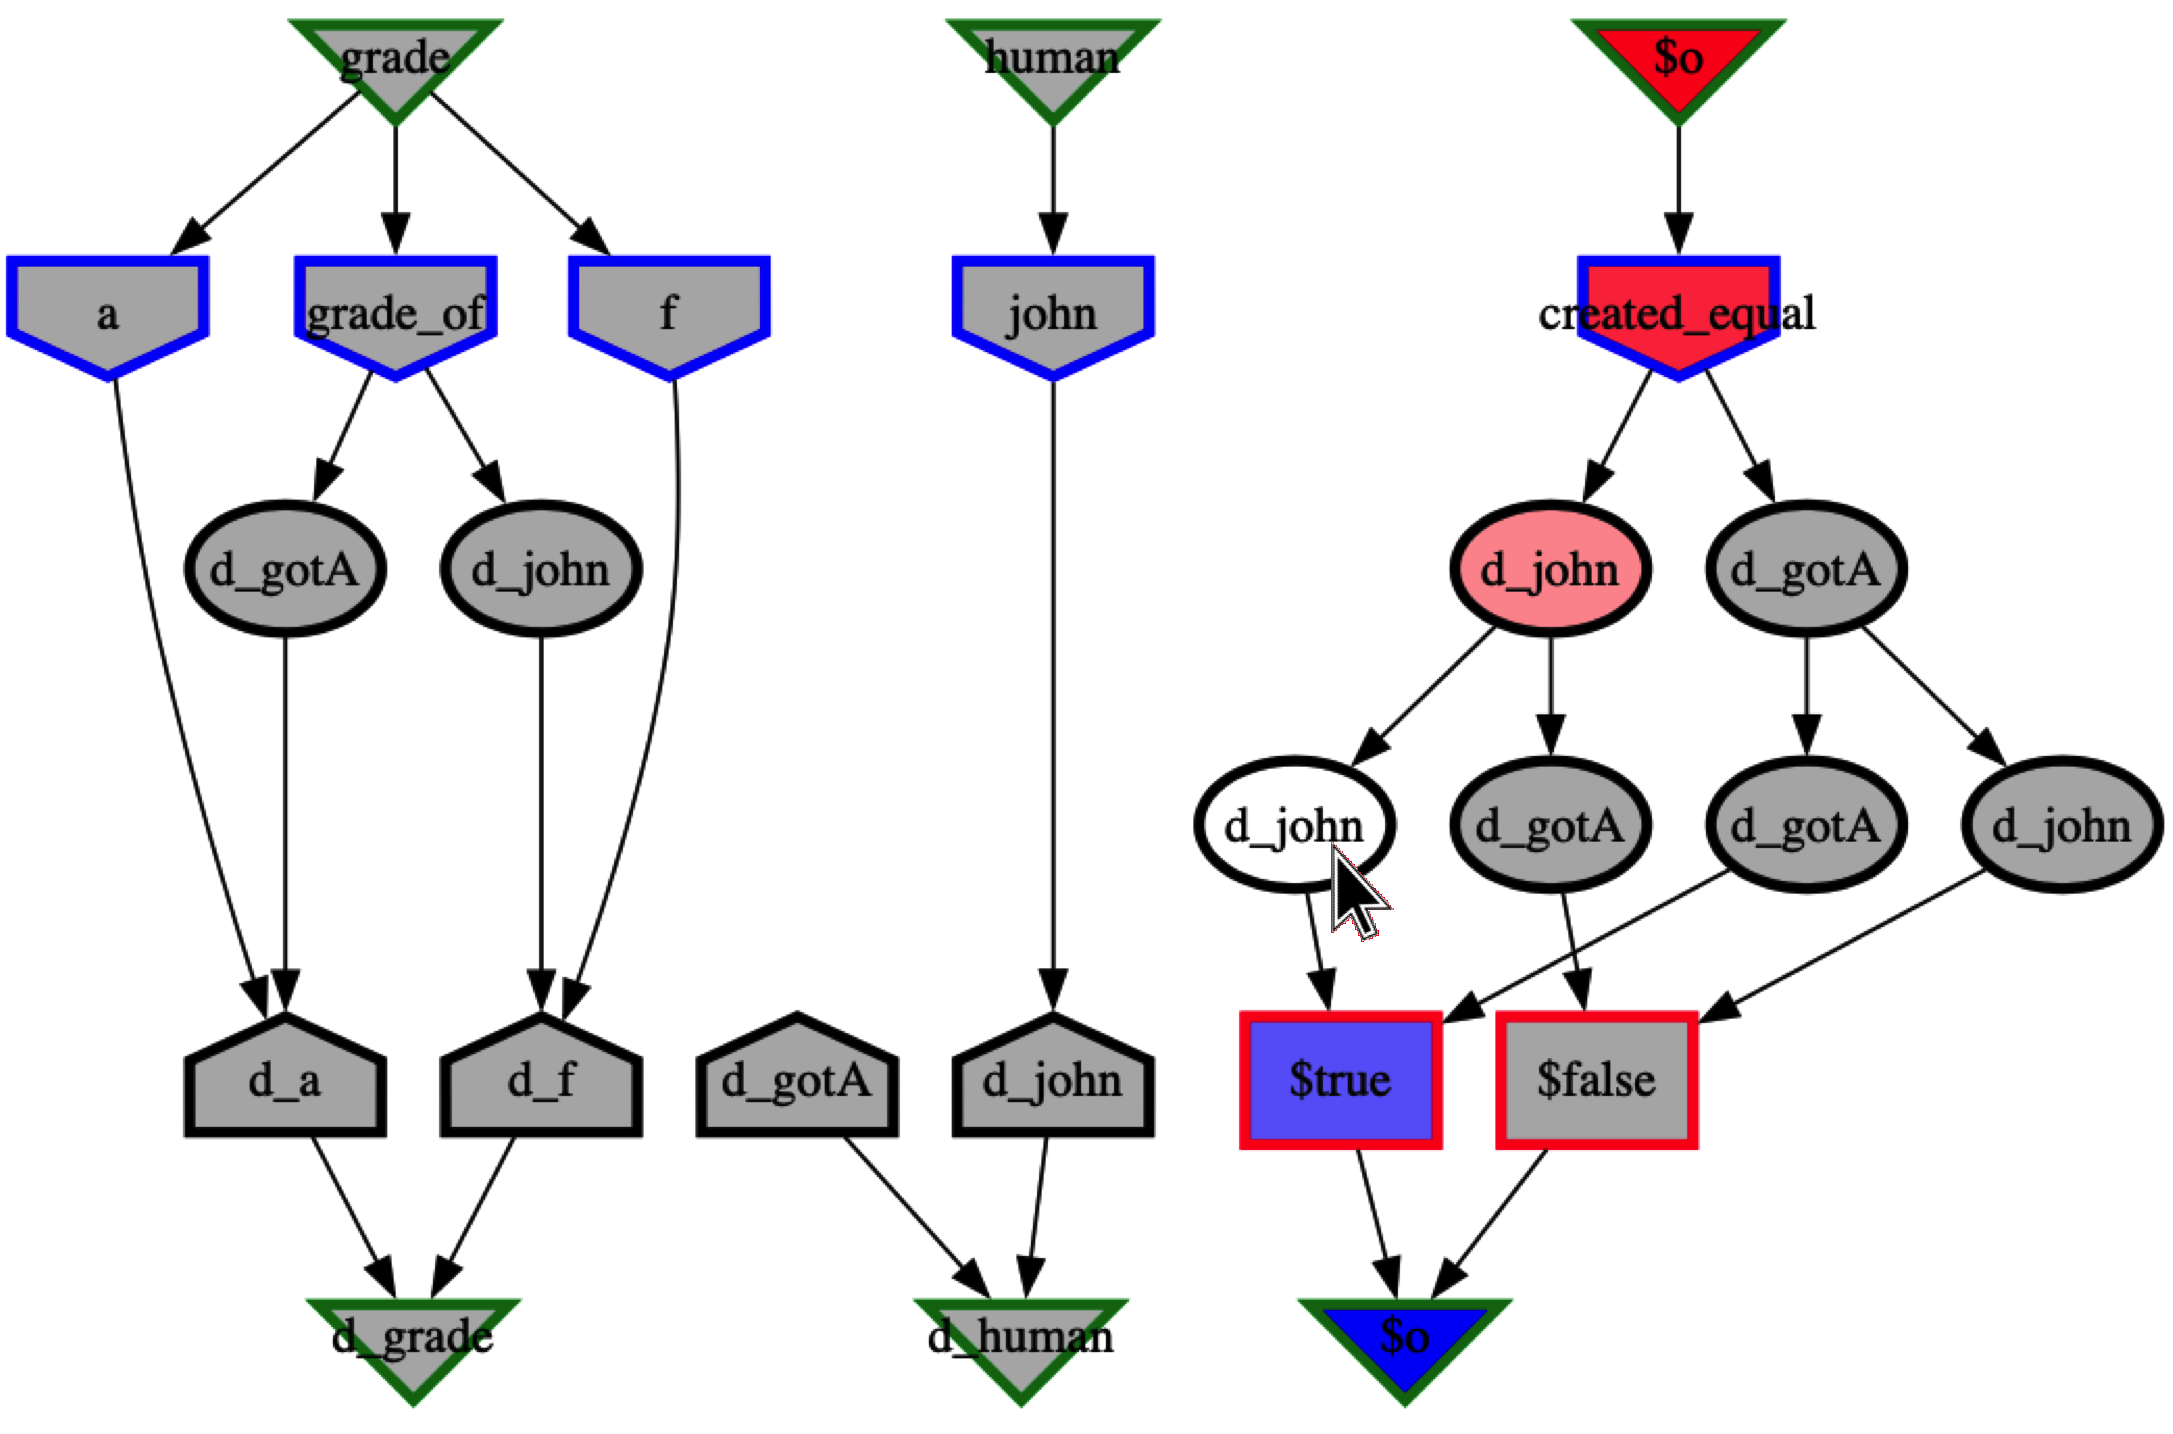
\includegraphics[width=\columnwidth]{TFF_Finite.s.IIV.pdf}
\caption{Visualization of the interpretation in Figure~\ref{TF0FiniteInterpretation}}
\label{TF0FiniteIIV}
\end{figure}

Further inspiration might lead to improvements to these visualizations, especially for more
complex infinite interpretations.

%--------------------------------------------------------------------------------------------------
\section{Conclusion}
\label{Conclusion}

This poster describes 

%--------------------------------------------------------------------------------------------------
\bibliographystyle{flairs}
\bibliography{Bibliography.bib}
%--------------------------------------------------------------------------------------------------
\end{document}
%--------------------------------------------------------------------------------------------------
%% \section{Formatting Requirements in Brief}
%% We need source and PDF files that can be used in a variety of ways and can be output on a variety of devices. FLAIRS imposes some requirements on your source and PDF files that must be followed. Most of these requirements are based on our efforts to standardize conference manuscript properties and layout. These requirements are as follows, and all papers submitted to FLAIRS for publication must comply:
%% 
%% \begin{itemize}
%% \item Your .tex file must compile in PDF\LaTeX{} --- \textbf{ no .ps or .eps figure files.}
%% \item All fonts must be embedded in the PDF file --- \textbf{ this includes your figures.}
%% \item Modifications to the style sheet (or your document) in an effort to avoid extra page  are NOT allowed.
%% \item No type 3 fonts may be used (even in illustrations).
%% \item Your title must follow US capitalization rules.
%% \item \LaTeX{} documents must use the Times or Nimbus font package (do not use Computer Modern for the text of your paper).
%% \item Fonts that require non-English language support (CID and Identity-H) must be converted to outlines or removed from the document (even if they are in a graphics file embedded in the document). 
%% \item Two-column format is required for all papers.
%% \item The paper size for final submission must be US letter. No exceptions.
%% \item The source file must exactly match the PDF.
%% \item The document margins must be as specified in the formatting instructions.
%% \item The number of pages and the file size must be as specified for your event.
%% \item No document may be password protected.
%% \item Neither the PDFs nor the source may contain any embedded links or bookmarks.
%% \item Your source and PDF must not have any page numbers, footers, or headers.
%% \item Your PDF must be compatible with Acrobat 5 or higher.
%% \item Your \LaTeX{} source file (excluding references) must consist of a \textbf{single} file (use of the ``input" command is not allowed.
%% \item Your graphics must be sized appropriately outside of \LaTeX{} (do not use the ``clip" command) .
%% \end{itemize}
%% 
%% If you do not follow the above requirements, it is likely that we will be unable to publish your paper.
%% 
%% \section{What Files to Submit}
%% You must submit the following items to ensure that your paper is published:
%% \begin{itemize}
%% \item A fully-compliant PDF file.
%% \item Your  \LaTeX{}  source file submitted as a \textbf{single} .tex file (do not use the ``input" command to include sections of your paper --- every section must be in the single source file). The only exception is the bibliography, which you may include separately. Your source must compile on our system, which includes the standard \LaTeX{} support files.
%% \item All your graphics files.
%% \item The \LaTeX{}-generated files (e.g. .aux and .bib file, etc.) for your compiled source.
%% \item All the nonstandard style files (ones not commonly found in standard \LaTeX{} installations) used in your document (including, for example, old algorithm style files). If in doubt, include it.
%% \end{itemize}
%% 
%% Your \LaTeX{} source will be reviewed and recompiled on our system (if it does not compile, you may incur late fees).   \textbf{Do not submit your source in multiple text files.} Your single \LaTeX{} source file must include all your text, your bibliography (formatted using flairs.bst), and any custom macros. Accompanying this source file, you must also supply any nonstandard (or older) referenced style files and all your referenced graphics files. 
%% 
%% Your files should work without any supporting files (other than the program itself) on any computer with a standard \LaTeX{} distribution. Place your PDF and source files in a single tar, zipped, gzipped, stuffed, or compressed archive. Name your source file with your last (family) name.
%% 
%% \textbf{Do not send files that are not actually used in the paper.} We don't want you to send us any files not needed for compiling your paper, including, for example, this instructions file, unused graphics files, and so forth.  
%% 
%% \section{Using \LaTeX{} to Format Your Paper}
%% 
%% The latest version of the FLAIRS style file is available on FLAIRS's website. Download this file and place it in a file named ``flairs.sty" in the \TeX\ search path. Placing it in the same directory as the paper should also work. You must download the latest version.
%% 
%% The following packages are incompatible with flairs.sty and/or flairs.bst and must not be used (this list is not exhaustive --- there are others as well):
%% \begin{itemize}
%% \item hyperref
%% \item natbib
%% \item geometry
%% \item titlesec
%% \item layout
%% \item caption
%% \item titlesec
%% \item T1 fontenc package (install the CM super fonts package instead)
%% \end{itemize}
%% 
%% \subsection{Illegal Commands}
%% The following commands may not be used in your paper:
%% \begin{itemize}
%% \item \textbackslash input
%% \item \textbackslash vspace (when used before or after a section or subsection)
%% \item \textbackslash addtolength 
%% \item \textbackslash columnsep
%% \item \textbackslash top margin (or text height or addsidemargin or even side margin)
%% \end{itemize}
%% 
%% \subsection{Paper Size, Margins, and Column Width}
%% Papers must be formatted to print in two-column format on 8.5 x 11 inch US letter-sized paper. The margins must be exactly as follows: 
%% \begin{itemize}
%% \item Top margin: .75 inches
%% \item Left margin: .75 inches
%% \item Right margin: .75 inches
%% \item Bottom margin: 1.25 inches
%% \end{itemize} 
%% 
%% 
%% The default paper size in most installations of \LaTeX{} is A4. However, because we require that your electronic paper be formatted in US letter size, you will need to alter the default for this paper to US letter size. Assuming you are using the 2e version of \LaTeX{}, you can do this by including the [letterpaper] option at the beginning of your file: 
%% \textbackslash documentclass[letterpaper]{article}. 
%% 
%% This command is usually sufficient to change the format. Sometimes, however, it may not work. Use PDF\LaTeX{} and include
%% \textbackslash setlength\{\textbackslash pdfpagewidth\}\{8.5in\}
%% \textbackslash setlength\{\textbackslash pdfpageheight\}\{11in\}
%% in your preamble. 
%% 
%% \textbf{Do not use the Geometry package to alter the page size.} Use of this style file alters flairs.sty and will result in your paper being rejected. 
%% 
%% 
%% \subsubsection{Column Width and Margins.}
%% To ensure maximum readability, your paper must include two columns. Each column should be 3.3 inches wide (slightly more than 3.25 inches), with a .375 inch (.952 cm) gutter of white space between the two columns. The flairs.sty file will automatically create these columns for you. 
%% 
%% \subsection{Overlength Papers}
%% If your paper is too long, turn on \textbackslash frenchspacing, which will reduce the space after periods. Next,  shrink the size of your graphics. Use \textbackslash centering instead of \textbackslash begin\{center\} in your figure environment. If these two methods don't work, you may minimally use the following. For floats (tables and figures), you may minimally reduce \textbackslash floatsep, \textbackslash textfloatsep, \textbackslash abovecaptionskip, and \textbackslash belowcaptionskip. For mathematical environments, you may minimally reduce \textbackslash abovedisplayskip, \textbackslash belowdisplayskip, and \textbackslash arraycolsep. You may also alter the size of your bibliography by inserting \textbackslash fontsize\{9.5pt\}\{10.5pt\} \textbackslash selectfont
%% right before the bibliography. 
%% 
%% Commands that alter page layout are forbidden. These include \textbackslash columnsep, \textbackslash topmargin, \textbackslash topskip, \textbackslash textheight, \textbackslash textwidth, \textbackslash oddsidemargin, and \textbackslash evensizemargin (this list is not exhaustive). If you alter page layout, you will be required to pay the page fee \textit{plus} a reformatting fee. Other commands that are questionable and may cause your paper to be rejected include  \textbackslash parindent, and \textbackslash parskip. Commands that alter the space between sections are also questionable. The title sec package is not allowed. Regardless of the above, if your paper is obviously ``squeezed" it is not going to to be accepted. Before using every trick you know to make your paper a certain length, try reducing the size of your graphics or cutting text instead.
%% 
%% \subsection{Credits}
%% Any credits to a sponsoring agency should appear in the acknowledgments section, unless the agency requires different placement. If it is necessary to include this information on the front page, use
%% \textbackslash thanks in either the \textbackslash author or \textbackslash title commands.
%% For example:
%% \begin{quote}
%% \begin{small}
%% \textbackslash title\{Very Important Results in AI\textbackslash thanks\{This work is
%%  supported by everybody.\}\}
%% \end{small}
%% \end{quote}
%% Multiple \textbackslash thanks commands can be given. Each will result in a separate footnote indication in the author or title with the corresponding text at the botton of the first column of the document. Note that the \textbackslash thanks command is fragile. You will need to use \textbackslash protect.
%% 
%% Please do not include \textbackslash pubnote commands in your document.
%% 
